\chapter{Introduzione}
\section{Cos'è la complessità computazionale?}

La Teoria della Complessità pone domande fondamentali sullo studio dei problemi
computazionali, cercando di comprendere la natura e le sfide che questi rappresentano.
Le questioni centrali che guida la ricerca in questo campo includono:

\begin{itemize}
    \item Come le risorse necessarie per risolvere un problema si scalano con una misura
    della dimensione del problema?
    \item Perché alcuni problemi sono difficili e altri facili?
    \item Cosa rende i problemi difficili, ``difficili''?
    \item Perché tutto ciò è importante per noi?
\end{itemize}

Queste domande ci aiutano a capire non solo la natura dei problemi computazionali
ma anche come e perché alcune questioni sono intrinsecamente più complesse di altre.
Esplorando queste domande, la Teoria della Complessità ci fornisce strumenti e metriche
per valutare e confrontare problemi computazionali, gettando luce sui limiti del calcolo
e sull'efficacia degli algoritmi.

\begin{pastelbox1}[title=Definizione di Complessità Computazionale]
    La Complessità Computazionale è lo studio delle risorse necessarie per risolvere
    problemi computazionali.
\end{pastelbox1}

\subsection{Primi problemi computazionali}
Supponiamo di di avere il seguente grafo:
\begin{figure}[H]
    \centering 
    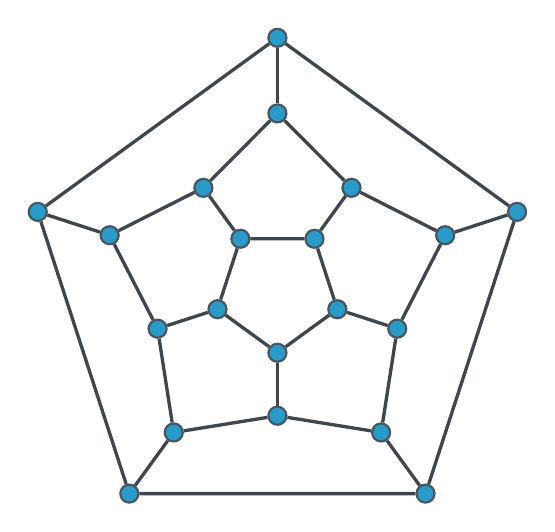
\begin{tikzpicture}[scale=1.6]
        \begin{scope}
            \tikzset{unode/.style = {
                circle, 
                draw=cyan!30!black, 
                thick,
                fill=cyan!80!black,
                inner sep=2.3pt,
                minimum size=2.3pt } }
            \tikzset{uedge/.style = {
                draw=cyan!20!black, 
                very thick} }
                \foreach \x in {0,1,2,3,4}{
                    \node[unode] (o\x) at (18+\x*72:2cm) {};
                    \node[unode] (i\x) at (18+\x*72:1.4cm) {};
                    \node[unode] (ii\x) at (54+\x*72:1cm) {};
                    \node[unode] (iii\x) at (54+\x*72:0.5cm) {};
                }
                \foreach \x in {0,1,2,3,4}{
                    \path[uedge] (o\x) edge (i\x); 
                    \path[uedge] (ii\x) edge (iii\x);
                }
                \path[uedge] (o0)--(o1)--(o2)--(o3)--(o4)--(o0);
                \path[uedge] (iii0)--(iii1)--(iii2)--(iii3)--(iii4)--(iii0);
                \path[uedge] (i0)--(ii0)--(i1)--(ii1)--(i2)--(ii2)--(i3)--(ii3)--(i4)--(ii4)--(i0);
        \end{scope}
    \end{tikzpicture}
\end{figure}
Supponiamo di voler risolvere questi due problemi:
\begin{itemize}
    \item C'è un cammino del grafo $\mathcal{G}$ che tocca tutti gli archi 
    esattamente una volta?
    \item C'è un cammino del grafo $\mathcal{G}$ che tocca tutti i nodi
    esattamente una volta?
\end{itemize}
Il primo problema è noto come \textbf{Problema del Ciclo Euleriano}, mentre il secondo
è noto come \textbf{Problema del Cammino Hamiltoniano}.

\subsection{Il Ciclo Euleriano}
Il problema del Ciclo Euleriano è stato formulato da Leonhard Euler nel 1736, quando risolse il problema dei ponti di Königsberg. Il problema consisteva nel trovare un percorso che attraversasse ogni ponte della città esattamente una volta senza ripercorrere lo stesso ponte.

\begin{figure}[ht]
    \centering
    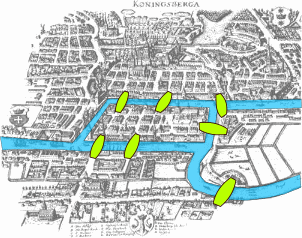
\includegraphics[width=0.5\textwidth]{img/Konigsberg_bridges.png}
    \caption{I ponti di Königsberg}
    \label{fig:konigsberg_bridges}
\end{figure}

Euler riuscì a trasformare questo problema pratico in un quesito astratto di teoria dei grafi. Sostanzialmente, il problema chiede se esiste un ciclo in un grafo che attraversi tutti gli archi esattamente una volta. Euler formulò un teorema, che descrive le condizioni necessarie affinché esista tale ciclo.

\begin{pastelbox2}[title=Teorema di Euler]
    Un grafo connesso e non orientato possiede un ciclo che inizia e termina sullo
    stesso vertice e attraversa ogni arco esattamente una volta se e solo se ogni
    vertice ha grado pari. Se ci sono esattamente due vertici di grado dispari, allora
    esiste un percorso che inizia in un vertice, attraversa ogni arco esattamente una volta,
    e termina nell'altro vertice.
\end{pastelbox2}
Euler dimostrò che un grafo ha un ciclo euleriano se e solo se è connesso e
ogni nodo ha un grado pari. Se il grafo non è connesso, o se ha più di due nodi
con un grado dispari, allora non può avere un ciclo euleriano. Questo risultato non
solo ha risolto il problema dei ponti di Königsberg ma ha anche gettato le basi per il
campo della teoria dei grafi.

Il costo computazionale per \textbf{decidere} se un grafo ha un ciclo euleriano è
$O(|V|+|E|)$, dove $|V|$ è il numero di nodi e $|E|$ è il numero di archi. 

\begin{algorithm}[H]
    \SetAlgoLined
    \SetKwInOut{Input}{Input}
    \SetKwInOut{Output}{Output}
    \SetKwFunction{FMain}{Main}
    \SetKwProg{Fn}{Function}{:}{}
    \SetKwProg{Pn}{Program}{:}{\KwRet}
    
    \DontPrintSemicolon
    \caption{Determinazione di un ciclo euleriano in un grafo $\mathcal{G}$}
    \label{alg:eulero_algo}
    
    \Input{Un grafo connesso e non orientato $\mathcal{G}$}
    \Output{Booleano che indica se il grafo $\mathcal{G}$ ha un ciclo euleriano}
    
    \BlankLine
    $\texttt{odd-vertex-num} \gets 0$\;
    \ForEach{$v \in \mathcal{G}.V$}{
        \If{$\texttt{degree}(v) \mod 2 \neq 0$}{
            $\texttt{odd-vertex-num} \gets \texttt{odd-vertex-num} + 1$\;
        }
    }
    \If{$\texttt{odd-vertex-num} = 0 \lor \texttt{odd-vertex-num} = 2$}{
        \Return \texttt{true}\;
    }
    \Return \texttt{false}\;
\end{algorithm}

Ci chiediamo ora quanto costa \textbf{certificare} che il grafo $\mathcal{G}$
ha un ciclo euleriano.
La complessità computazionale per certificare che un grafo ha un ciclo
euleriano è $O(|V|+|E|)$, dove $|V|$ è il numero di nodi e $|E|$ è il numero di archi.
Questo perché ci basterebbe scorrere il grafo e contare il grado di ogni nodo.

\subsection{Il Cammino Hamiltoniano e il Ciclo Hamiltoniano}
Proprio come il problema dei ponti di Königsberg ha portato alla definizione del ciclo
euleriano, la ricerca di un ciclo che visiti ogni vertice di un grafo esattamente
una volta ha portato alla definizione di un ciclo hamiltoniano. Questo problema
prende il nome dal matematico William Rowan Hamilton che lo studiò nel XIX secolo.

A differenza dei cicli euleriani, dove un ciclo deve attraversare tutti gli archi
esattamente una volta, un ciclo hamiltoniano deve passare per tutti i vertici una
sola volta e tornare al vertice di partenza. Il problema del ciclo hamiltoniano
chiede se tale ciclo esista in un dato grafo.

\begin{pastelbox3}[title=Problema del Ciclo Hamiltoniano]
    Un ciclo hamiltoniano esiste in un grafo $\mathcal{G}$ se e solo se esiste una
    sequenza chiusa che
    visita ogni vertice una volta prima di ritornare al vertice iniziale. Tuttavia, a
    differenza del problema euleriano, non esiste un criterio semplice per verificare
    l'esistenza di un ciclo hamiltoniano in un grafo generale.
\end{pastelbox3}

Il problema del ciclo hamiltoniano è \texttt{NP-completo}, il che significa che non è noto
alcun algoritmo efficiente che lo risolva per ogni grafo in tempo polinomiale.
È interessante notare che, mentre per i cicli euleriani è relativamente semplice
determinarne l'esistenza e costruirli, per i cicli hamiltoniani anche solo la verifica
della loro esistenza può essere computazionalmente impegnativa.

Quanto costa \textbf{decidere} se un grafo $\mathcal{G}$ è hamiltoniano? Non lo sappiamo
con certezza! Forse richiede tempo esponenziale? Quanto costa \textbf{verificare}
che un grafo $G$ sia o non sia hamiltoniano? Per mostrare che lo è, basta fornire un
cammino hamiltoniano.

\subsection{Il Problema della partizione massima}

Consideriamo i seguenti 38 numeri. La loro somma è 2 000 000: 

\begin{verbatim}
14175 15055 16616 17495 18072 19390 19731 22161 23320 23717 
26343 28725 29127 32257 40020 41867 43155 46298 56734 57176 
58306 61848 65825 66042 68634 69189 72936 74287 74537 81942 
82027 82623 82802 82988 90467 97042 97507 99564
\end{verbatim}

Per verificare una potenziale soluzione a questo problema, si potrebbe pensare di provare
tutte le possibili combinazioni dei 38 numeri presi 19 alla volta. Questo approccio,
tuttavia, comporterebbe l'esplorazione di circa $35 \times 10^9$ configurazioni diverse,
un compito computazionalmente oneroso.

Se, invece, vi fosse data una specifica partizione dei numeri, il costo per verificarne
la validità sarebbe notevolmente inferiore. Per confermare che una partizione proposta è una soluzione valida, sarebbe sufficiente:

\begin{enumerate}
    \item Assicurarsi che ciascun gruppo sia composto esattamente da $19$ numeri.
    \item Sommare i numeri in uno dei gruppi per verificare che la loro somma sia
    pari a $1000000$.
\end{enumerate}

Questa metodologia di verifica fornisce un modo efficiente per confermare la correttezza
di una soluzione proposta senza la necessità di esaminare tutte le possibili combinazioni.

\subsection{La Primalità di un Numero e la Ricerca di Fattori Piccoli}
Un problema fondamentale nell'aritmetica e nella crittografia è determinare se un numero
intero $N$ sia primo o meno. Inoltre, si può voler sapere se $N$ ha un fattore piccolo,
inferiore a un certo limite $q$. 

Un esempio storico notevole fu presentato da Frank Cole nel $1903$, quando dimostrò che:
\[N = 193707721 \times 761838257287\]
scomponendo così il numero in due fattori primi, senza l'ausilio di computer o calcolatrici elettroniche, ma probabilmente mediante metodi sistematici e molta pazienza.

\subsubsection{Algoritmi per la Primalità}
L'algoritmo più efficiente conosciuto per decidere se un numero intero $N$ sia
primo ha una complessità temporale di $O((\log N)^{6+\epsilon})$, dove $\epsilon$ è
un piccolo numero positivo. Questo dimostra che, sebbene non sia immediato, il problema
della primalità può essere risolto in tempo polinomiale.

\subsubsection{Fattorizzazione:} 
D'altra parte, non conosciamo una procedura efficiente per
fattorizzare un grande intero nei suoi divisori, al di là del tentativo di tutte le
possibilità. Questo rende la fattorizzazione di grandi numeri una sfida significativa,
specialmente per i numeri che hanno solo fattori grandi.

\subsubsection{Costo della Certificazione di un Fattore Piccolo}
La certificazione o verifica di un fattore piccolo di $N$ può essere relativamente
semplice e rapida. Se ci viene dato un fattore $f < q$, possiamo semplicemente
dividere $N$ per $f$ e verificare se il risultato è un numero intero senza resto.
Questo processo ha un costo computazionale di $O(\log N)$, rendendolo efficiente
anche per numeri molto grandi.

Questa discussione evidenzia il contrasto tra la relativa facilità di verificare
la primalità o la presenza di fattori piccoli e la difficoltà significativa di
fattorizzare numeri grandi. Questo contrasto è al cuore di molti sistemi di
crittografia moderni, che si affidano alla difficoltà di fattorizzare come
garanzia di sicurezza.

\subsection{Il problema degli scacchi}
\begin{minipage}{0.5\textwidth}
    \begin{figure}[H]
        \centering
        \newchessgame 
        \chessboard[setfen=4r1b1/1p4B1/pN2pR2/RB2k3/1P2N2p/2P3b1/n2P1p1r/5K1n w - - 0 1,
            pgfstyle=straightmove,
            showmover=false]
        \caption{Scacco Matto in 3 mosse}
    \end{figure}
\end{minipage}%
\begin{minipage}{0.5\textwidth}
    \begin{figure}[H]
        \centering
        \newchessgame 
        \chessboard[setfen=6N1/5KR1/2n5/8/8/8/2n5/1k6 w - - 0 1,
            pgfstyle=straightmove,
            showmover=false]
        \caption{Scacco Matto in 262 mosse}
    \end{figure}
\end{minipage}

Un aspetto interessante degli scacchi è la verifica della presenza di uno scacco
matto in una data posizione. La complessità di tale verifica aumenta con il numero
di mosse necessarie per raggiungere lo scacco matto dallo stato attuale della scacchiera.
Consideriamo il seguente ragionamento logico per dimostrare uno scacco matto in $n$ mosse:

\textit{``Esiste una mossa $w_1$ tale che, per qualsiasi risposta $b_1$, esiste una mossa
$w_2$ tale che, per qualsiasi risposta $b_2$, ..., fino a che per qualsiasi risposta
$b_{n-1}$, esiste una mossa $w_n$ che produce uno scacco matto."}

Questo implica una sequenza di mosse forzate in cui il Bianco, indipendentemente dalle
mosse del Nero, può garantire uno scacco matto. Tale sequenza di mosse è spesso indicata
come ``matto in $n$ mosse". Il processo di verifica di questa affermazione richiede una
conoscenza approfondita delle strategie di scacchi e, per posizioni complesse, può
richiedere molto tempo.

\section{Problema computazionale}
\begin{pastelbox4}[title=Problema computazionale]
    Un problema computazionale descrive un infinito insieme di possibili input,
    chiamati \textit{istanze}, e rappresenta una relazione che mappa ogni istanza a
    un insieme non vuoto di possibili output.
\end{pastelbox4}
Questa definizione sottolinea due componenti fondamentali di un problema computazionale:
\begin{itemize}
    \item \textbf{Insieme di Istanze}: Ogni problema computazionale ammette un'infinità di possibili istanze di input. Queste istanze rappresentano le diverse configurazioni o scenari su cui il problema può operare.
    \item \textbf{Relazione Input-Output}: Per ogni istanza di input, esiste una relazione ben definita che determina l'insieme dei possibili output. Questa relazione è cruciale per definire correttamente il problema e per comprendere la natura delle soluzioni possibili.
\end{itemize}
Un problema computazionale non è una singola domanda, ma una famiglia 
di domande, ognuna delle quali corrisponde a una diversa istanza di input.
\subsection{Misurazione dell'efficienza algoritmica}

L'efficienza di un algoritmo nel risolvere un problema computazionale è fondamentale
per comprendere sia la sua praticità sia la sua applicabilità a insiemi di dati di
grandi dimensioni. La misurazione dell'efficienza algoritmica si basa su diversi
fattori chiave:

\begin{itemize}
    \item \textbf{Dimensione dell'istanza (\(n\))}: Rappresenta la quantità di dati
    in input all'algoritmo. La dimensione dell'istanza è spesso il fattore più diretto
    che influenza la complessità di un problema.
    \item \textbf{Crescita delle risorse utilizzate (\(T(n)\))}: Indica come le risorse
    necessarie per eseguire l'algoritmo crescono con l'aumentare della dimensione
    dell'input. \(T(n)\) è spesso espressa in termini di tempo (\textit{ad esempio, il numero
    di operazioni richieste}) o spazio (\textit{ad esempio, la quantità di memoria necessaria}).
    \item \textbf{Caso peggiore}: Analizza la complessità dell'algoritmo nella situazione
    più sfavorevole possibile. Questo scenario fornisce un limite superiore sulle risorse
    necessarie per qualsiasi input di dimensione \(n\).
\end{itemize}

Anche se non trattato qui, è importante notare che, oltre al caso peggiore, si può
considerare anche il caso medio, che fornisce un'indicazione delle risorse necessarie
in media, dato un insieme rappresentativo di istanze di input.

Questa analisi permette di valutare e confrontare algoritmi in base alla loro efficienza,
guidando la scelta dell'algoritmo più adatto per un determinato problema e insieme di dati.

\subsection{Complessità computazionale}

La \textbf{complessità computazionale} si riferisce alla quantità di risorse
computazionali necessarie per risolvere il problema in questione. La complessità può
essere esplorata sotto due principali prospettive: i limiti superiori e i limiti inferiori.

\subsubsection{Limiti Superiori}
I \textit{limiti superiori} indicano quanto bene possiamo risolvere il problema, cioè
la complessità dell'algoritmo più efficiente conosciuto che risolve il problema.
Dimostrare un limite superiore significa mostrare che esiste almeno un algoritmo
con la complessità affermata per risolvere il problema.

\subsubsection{Limiti Inferiori}
I \textit{limiti inferiori}, d'altra parte, indicano quanto sia difficile il problema,
ossia la quantità minima di risorse che ogni algoritmo deve utilizzare per risolverlo.
Per stabilire un limite inferiore, dobbiamo mostrare che tutti gli algoritmi hanno una
complessità almeno pari al limite inferiore affermato.

\subsubsection{Esempio}
Consideriamo il problema della moltiplicazione di due numeri interi di \(n\) cifre.
\begin{itemize}
    \item \textbf{Limiti Superiori:} La procedura elementare insegnata nelle scuole
    richiede \(O(n^2)\) moltiplicazioni ed addizioni elementari. Tuttavia, questo non
    è necessariamente la complessità del problema della moltiplicazione, poiché esistono
    algoritmi più efficienti.
    \item \textbf{Limiti Inferiori:} Al minimo, dobbiamo leggere tutto l'input, il che
    implica una complessità di almeno \(\Omega(n)\).
    \item L'\textit{algoritmo di Karatsuba} riduce la complessità a
    \(O(n^{\log_2 3}) = O(n^{1.585})\), dimostrando che la moltiplicazione può essere
    effettuata più velocemente rispetto alla procedura elementare.
    \item L'\textit{algoritmo migliore conosciuto} per la moltiplicazione ha una
    complessità inferiore a \(o(n^{1+\epsilon})\) per ogni \(\epsilon > 0\), dove
    la notazione \(o(\cdot)\) indica una crescita asintotica più lenta rispetto alla
    funzione dentro le parentesi.
\end{itemize}

Questo esempio illustra come l'analisi della complessità fornisca una comprensione
profonda sia delle potenzialità sia dei limiti degli algoritmi nel risolvere problemi
computazionali.

\subsection{Trattabilità di un problema}
La comprensione della differenza tra \textbf{crescita polinomiale} e \textbf{crescita esponenziale}
delle risorse necessarie da un algoritmo è fondamentale per valutare la sua efficienza e praticabilità.
Jack Edmonds, nel 1965, ha sottolineato l'importanza di questa distinzione, che rimane centrale
nell'analisi degli algoritmi.

\subsubsection{Crescita Polinomiale}
La crescita polinomiale si verifica quando il requisito di risorse di un algoritmo è limitato
da \(n^k\) per qualche costante \(k\). In questo contesto, se l'input raddoppia da \(n\) a \(2n\),
il requisito di risorse aumenta di un fattore costante, da \(n^k\) a \(2^k n^k\). Questo indica che
la crescita delle risorse necessarie è gestibile e prevedibile al crescere delle dimensioni dell'input.

\subsubsection{Crescita Esponenziale}
Al contrario, la crescita esponenziale descrive una situazione in cui il requisito di risorse cresce
proporzionalmente a \(c^n\) per qualche costante \(c > 1\). Quando l'input raddoppia, il requisito di
risorse si quadruplica, passando da \(c^n\) a \(c^{2n} = (c^n)^2\). Questa rapida escalation rende gli
algoritmi con crescita esponenziale impraticabili per input di grandi dimensioni.

\begin{figure}[H]
    \centering
    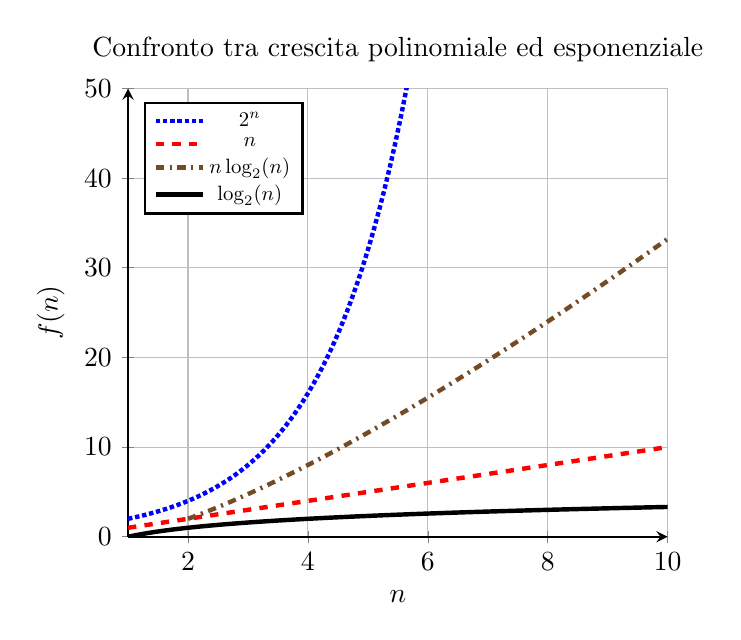
\begin{tikzpicture}
        \begin{axis}[
            axis lines=left,
            title={Confronto tra crescita polinomiale ed esponenziale},
            xlabel={$n$},
            ylabel={$f(n)$},
            ymin=0, ymax=50, 
            xmin=1, xmax=10,
            domain=1:10,
            samples=100, 
            no markers,
            thick,
            grid=both,
            legend pos=north west,
            legend style={nodes={scale=0.75, transform shape}}
        ]

        % 2^n
        \addplot+[domain=1:10, style=densely dotted, ultra thick] {2^x};
        \addlegendentry{$2^n$};
        
        % n
        \addplot+[domain=1:10, style=dashed, ultra thick] {x};
        \addlegendentry{$n$};
        
        % n*log2(n)
        \addplot+[domain=2:10, style=dashdotted, ultra thick] {x*log2(x)};
        \addlegendentry{$n \log_2(n)$};
        
        % log2(n)
        \addplot+[domain=1:10, style=solid, ultra thick] {log2(x)};
        \addlegendentry{$\log_2(n)$};
        
        \end{axis}
    \end{tikzpicture}
\end{figure}
\begin{pastelbox1}[title=Legge di Moore]
    La legge di Moore, formulata da Gordon Moore nel 1965, afferma che il numero di transistor
    in un microprocessore raddoppia approssimativamente ogni 18 mesi.
\end{pastelbox1}
Ogni due anni la velocità dei computer raddoppia, ma questo non è sempre decisivo.
Consideriamo due scenari:
    
\subsubsection*{Algoritmi Polinomiali: \(O(n^k)\)}
Con un algoritmo polinomiale, il tempo di esecuzione cresce polinomialmente con la
dimensione dell'input \(n\). In un tempo \(T\):
\begin{itemize}
    \item Se oggi risolviamo istanze di dimensione \(n_T\),
    \item tra due anni possiamo risolvere istanze di dimensione \(n' = n_T 2^{1/k}\).
\end{itemize}
Questo dimostra che l'aumento di potenza computazionale ci permette di gestire istanze
significativamente più grandi in modo più efficiente.
    
\subsubsection{Algoritmi Esponenziali: \(\Omega(2^n)\)}
Con un algoritmo esponenziale, il tempo di esecuzione cresce esponenzialmente con la dimensione
dell'input \(n\). In un tempo \(T\):
\begin{itemize}
    \item Se oggi risolviamo istanze di dimensione \(n_T\),
    \item tra due anni possiamo risolvere istanze di dimensione \(n' = n_T + 1\).
\end{itemize}
In questo caso, l'aumento di potenza computazionale ci consente di affrontare solo istanze
leggermente più grandi, evidenziando i limiti degli algoritmi con crescita esponenziale.